%!TEX root = IntroArithGrps.tex

\mychapter{\texorpdfstring{Geometric Meaning of\\$\real$-rank and $\rational$-rank}%
	{Geometric Meaning of R-rank and Q-rank}}
\label{GeomIntroRank}

\prereqs{locally symmetric spaces (\cref{WhatisLocSymmChap}) and other differential geometry.}

This chapter, like the previous one, is motivational. It is not a
prerequisite for later chapters.



\section{Rank and real rank} \label{IntroRrankSect}

Let $X$ be a symmetric space \csee{symmDefn}. 
%(That is, for each point $p \in X$, there is an isometry $\phi$ of~$X$, such that the derivative $d \phi_p$ is $-\Id$ on the tangent space $T_p X$.) 
For example, $X$ could
be a Euclidean space $\real^n$, or a round sphere $S^n$, or a hyperbolic
space $\hyperbolic^n$, or a product of any combination of these.


As is well known, the rank of~$X$ is a natural number that
describes part of the geometry of~$X$, namely, the
dimension of a maximal flat.

\begin{defn}
 A \defit[flat!in a symmetric space]{flat} in~$X$ is a connected, totally geodesic,
flat submanifold of~$X$.
 \end{defn}

\begin{defn}
	\nindex{$\rank X$ = dimension of maximal flat}%
 $\rank X$ is the largest natural number~$r$, such that
$X$ contains an $r$-dimensional flat.
 \end{defn}

Let us assume that $X$ has no flat factors. (That is, the universal
cover of~$X$ is not isometric to a product of the form $Y \times
\real^n$. Mostly, we will be interested in the case where
$X$ also does not have any compact factors.)

Let $G = \Isom(X)^\circ$. Then $G$ acts transitively on~$X$, and there
is a compact subgroup~$K$ of~$G$, such that $X = G/K$. Because $X$ has no
flat factors, $G$ is a connected, semisimple, real Lie group with
trivial center (see~\S\ref{ConstructSymm}). (We remark that $G$ is
isomorphic to a closed subgroup of $\SL(\ell,\real)$, for some~$\ell$.)

The real rank can be understood similarly. It is an invariant of~$G$
that is defined algebraically \csee{RrankChap}, but it has the following geometric
interpretation.

\begin{thm} \label{Rrank-geometric}
	\nindex{$\Rrank G$ = maximal dimension of closed, simply connected flat}%
 $\Rrank G$ is the largest natural number~$r$, such that
$X$ contains a closed, \textbf{simply connected}, $r$-dimensional
flat.
 \end{thm}
 
\begin{warn}
By \emph{closed}, we simply mean that the flat contains all of its accumulation points, not that it is compact. (A closed, simply connected flat is homeomorphic to some Euclidean space~$\real^r$.)
\end{warn}

For example, if $X$ is compact, then every closed, totally
geodesic, flat subspace of~$X$ must be a torus,
not~$\real^n$, so $\Rrank G = 0$. On the other hand, if $X$
is not compact, then $X$ has unbounded geodesics (for
example, if $X$ is irreducible, then every geodesic goes to
infinity), so $\Rrank G \ge 1$. Hence:
 \centerline{$\Rrank G = 0
  \qquad\Leftrightarrow \qquad 
  \text{$X$~is compact}
 .$}
 Thus, there is a huge difference between $\Rrank G = 0$
and $\Rrank G > 0$, because no one would mistake a
compact space for a noncompact one.

\begin{rem}
 $\Rrank G = \rank X$ if and only if $X$ has no compact
factors.
 \end{rem}

There is also an important difference between $\Rrank G =
1$ and $\Rrank G > 1$. The following proposition is an important
example of this.

\begin{defn}
 $X$ is \defit{two-point homogeneous} if, whenever $(x_1,x_2)$ and
$(y_1,y_2)$ are two pairs of points in~$X$ with $d(x_1,x_2) =
d(y_1,y_2)$, there is an isometry~$g$ of~$X$ with $g(x_1) = y_1$ and
$g(x_2) = y_2$.
 \end{defn}

If $\Rrank G > 1$, then there exist maximal flats $H_1$ and~$H_2$ that
intersect nontrivially. On the other hand, there also exist some pairs
$x_1,x_2$, such that $\{x_1,x_2\}$ is not contained in the intersection
of any two (distinct) maximal flats. This establishes one direction of
the following result.

\begin{prop} \label{2ptHomog}
 Assume $X$ is noncompact and irreducible. The symmetric space~$X$ is
two-point homogeneous if and only if\/ $\Rrank G = 1$.
 \end{prop}

The following is an infinitesimal version of this result.

\begin{prop} \label{Rrank1->transitive}
 Assume $X$ is noncompact and irreducible. 
 The action of~$G$ on the set of unit tangent vectors
of~$X$ is transitive iff\/ $\Rrank G = 1$. 
 \end{prop}

\begin{cor}
 $\Rrank  \SO(1,n) = 1$.
 \end{cor}

\begin{proof}
 For $G = \SO(1,n)$, we have $X = \hyperbolic^n$. The stabilizer
$\SO(n)$ of a point in~$\hyperbolic^n$ acts transitively on the unit
tangent vectors at that point. So $G$ acts transitively on the unit
tangent vectors of~$X$.
 \end{proof}
 
More generally, it can be shown that $\Rrank \bigl( \SO(m,n) \bigr) = \min\{m,n\}$. Also,
$\Rrank \bigl( \SL(n,\real) \bigr) = n-1$. Although they may not be obvious geometrically, these real ranks are easy to calculate from the algebraic
definition that will be given in \cref{RrankChap}.

\begin{rem}
For every~$r$, there is a difference between $\Rrank G =
r$ and $\Rrank G > r$, but this difference is less
important as $r$~grows larger: the three main cases are
$\Rrank G = 0$, $\Rrank G = 1$, and $\Rrank G \ge 2$.
(This is analogous to the situation with smoothness
assumptions: countless theorems require a function to be
$C^0$ or $C^1$ or~$C^2$, but far fewer theorems require a
function to be, say,~$C^7$, rather than only~$C^6$.)
\end{rem}

%Real rank has the following implication for the geometry of
%$\Gamma \backslash X$:
%
%\begin{prop}
% Assume $X$ has no compact factors. Then:
% \begin{enumerate}
% \item There is a dense geodesic in $\Gamma \backslash X$.
% \item The geodesic flow on the unit tangent bundle $T^1(\Gamma
%\backslash X)$ has a dense orbit if and only if\/ $\Rrank G = 1$.
% \end{enumerate}
% \end{prop}

\begin{exercises}

\item Show $\Rrank(G_1 \times G_2) = \Rrank G_1 + \Rrank G_2$.

\item Assume $\Rrank G = 1$. Show $X$ is irreducible if and only if
$X$~has no compact factors.

\item Show that if $X$ is reducible, then $X$ is \emph{not} two-point
homogeneous. (Do not assume the fact about maximal flats that
was mentioned, without proof, before \cref{2ptHomog}.)

 \end{exercises}





\section{\texorpdfstring{$\rational$}{Q}-rank} \label{QrankIntroSect}

Now let $\Gamma \backslash X$ be a locally symmetric space
modeled on~$X$, and assume that
$\Gamma \backslash X$ has
finite volume. Hence, $\Gamma$ is a (torsion-free) discrete subgroup
of~$G$, such that $\Gamma \backslash G$ has finite volume;
in short, $\Gamma$ is a \defit[lattice!subgroup]{lattice} in~$G$.

The real rank depends only on~$X$, so it is not affected by the choice of
a particular lattice~$\Gamma$. We now describe an analogous
algebraically defined invariant, $\Qrank\Gamma$, that does depend
on~$\Gamma$, and therefore distinguishes between some of the various locally
homogeneous spaces that are modeled on~$X$. We will mention some of the
geometric implications of $\rational$-rank, leaving a more detailed
discussion to later chapters.

\begin{thm}[\csee{DivTorusSect,LargeScaleSect}] \label{QrankFlats} \ 
\noprelistbreak
\begin{enumerate}
 \item \label{QrankFlats-exists}
 $\Qrank\Gamma$ is the largest natural number~$r$, such
that some finite cover of\/ $\Gamma \backslash X$ contains a closed, simply connected,
$r$-dimensional flat.
\item \label{QrankFlats-BddDist}
$\Qrank\Gamma$ is the smallest natural number~$r$, for which there
exists collection of finitely many closed, $r$-dimensional flats, such that all of\/ $\Gamma \backslash X$ is within a bounded distance of the union of these flats. 
\end{enumerate}
 \end{thm}

\begin{rem} \label{QrankPossiblesMentioned}
 It is clear from \fullcref{QrankFlats}{exists}
that $\Qrank\Gamma$ always exists (and is finite). Furthermore,
$0 \le \Qrank\Gamma \le \Rrank G$. Although not so obvious, it can be shown that the extreme values are always
attained: there are lattices $\Gamma_c$ and~$\Gamma_s$ in~$G$ with
$\Qrank\Gamma_c = 0$ and $\Qrank\Gamma_s = \Rrank G$ \csee{GHasCpctLatt,Qrank=Rrank}. So it is
perhaps surprising that there may be gaps in between. 
(For example,  if $G \iso \SO(2,n)$, with $n \ge 5$, and
$n$~is odd, then $\Rrank G = 2$, but \cref{QrankGap} shows
there does not exist a lattice~$\Gamma$ in~$G$, such that $\Qrank\Gamma = 1$.)
 \end{rem}

\begin{eg}[\csee{QrankEg}] \label{QrankIntroEgs}
 From the algebraic definition, which will appear in
\cref{QrankChap}, it is easy to calculate 
 $$\Qrank \bigl( \SO(m,n)_{\integer} \bigr) = \min\{m,n\} = \Rrank \bigl(
\SO(m,n) \bigr)$$
 and 
 $$\Qrank \bigl( \SL(n,\integer) \bigr) = n-1 = \Rrank \bigl(
\SL(n,\real) \bigr) .$$
 \end{eg}

As for the real rank, the biggest difference is between spaces where the
invariant is zero and those where it is nonzero, because this is again
the distinction between a compact space and a noncompact one:

\begin{thm}[\csee{Qrank0Ex}] \label{Qrank0<>cocpct}
 $\Qrank\Gamma = 0$ iff\/ $\Gamma
\backslash X$~is compact.
 \end{thm}

\fullCref{QrankFlats}{BddDist} implies that the $\rational$-rank of~$\Gamma$ is
directly reflected in the large-scale geometry of~$\Gamma \backslash X$,
as described by the asymptotic cone of~$\Gamma \backslash X$.
 Intuitively, the asymptotic cone of a metric space is obtained
by looking at it from a large distance. For example, if $\Gamma
\backslash X$ is compact, then, as we move farther away, the manifold
appears smaller and smaller (see the illustration below). % !!! \csee{shrinkcpct}. 
In the limit, the manifold shrinks to a point.
\begin{align} \label{shrinkcpct} % cref calls this an equation, instead of a figure !!!
 \lower0.75\baselineskip\hbox{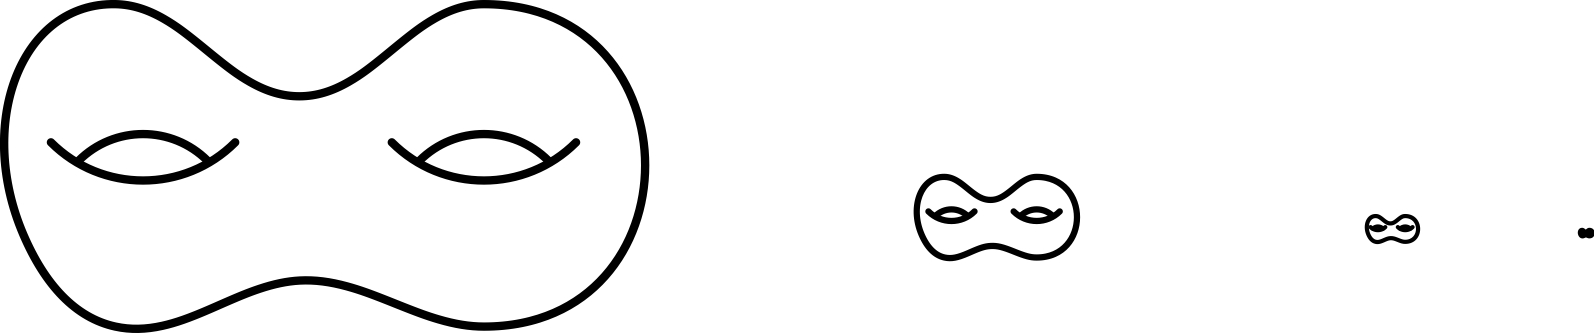
\includegraphics{PDF/shrinkcpct.jpg}}
\end{align}
%%%\begin{figure}[h]
%%% 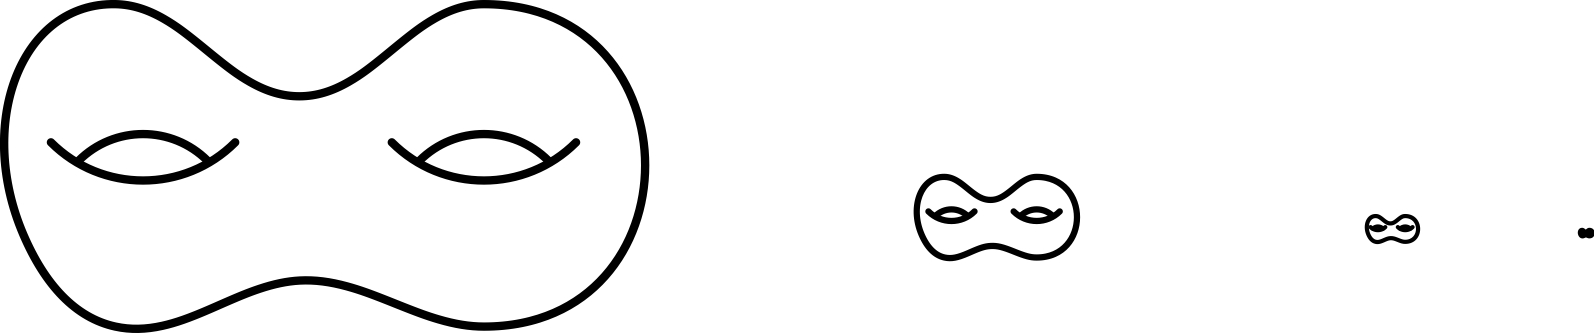
\includegraphics{PDF/shrinkcpct.jpg}
%%% \caption{Looking at a compact manifold from farther and farther away.}
%%%% \label{shrinkcpct}
%%% \end{figure}
%texpreamble
%("  \usepackage{amsmath}
% \usepackage[LY1]{fontenc}
% \usepackage[expert,LY1,mylucidascale]{mylucidabr}
% ");
%defaultpen(  fontcommand("\normalfont") + fontsize(10) ); 
%
%from graph access *;
%unitsize(0.39cm);
%
%currentpen = linewidth(1.25);
%
%void hole(real x, real s) {
%	draw( (x+s,s){SW}..{NW}(x-s, s) );
%	draw( (x+s*0.7,s*0.8){NW}..{SW}(x-s*0.7, s*0.8) );
%	}	
%
%
%void M(real m, real s, real thickness){
%	currentpen = linewidth(thickness);
%	draw( shift(m,0)* (scale(s)*((0,-1){W}..(-2,-0.5)..(-4,-1)..(-5,0)..(-4,2.5)..(-2,1.5)..{E}(0,2.5)
%		..{W}(0,-1) )));
%	hole(m,s); hole(m-3.7*s, s);
%	}
%
%M(0, 1, 1); 
%M(6, 0.25, 0.75);
%M(10, 0.08, 0.5);
%M(12, 0.02, 0.5);

An intuitive understanding is entirely sufficient for our purposes here,
but, for the interested reader, we provide a more formal definition.

\begin{defn} \label{AsympConeDefn}
 The \defit{asymptotic cone} of a metric space $(M,d)$ is the
limit space 
 $$\lim_{\epsilon \to 0^+} \bigl( (M, \epsilon d), p \bigr) ,$$
if the limit exists. Here, $p$ is an arbitrary (but fixed!) point of~$M$,
and the limit is with respect to Gromov's Hausdorff distance. (Roughly
speaking, a large ball around~$p$ in $(M, \epsilon d)$ is $\delta$-close
to being isometric to a large ball around a certain (fixed) point~$p_0$
in the limit space $(M_0,d_0)$.)
 \end{defn}

\begin{egs} \  \label{TanConeEgs}
\noprelistbreak
 \begin{enumerate}
 \item If $\Gamma \backslash X$ is compact, then the
asymptotic cone of $\Gamma \backslash X$ is a
point, as is illustrated in \pref{shrinkcpct}. This point is a $0$-dimensional simplicial
complex, which is a geometric manifestation of the
fact that $\Qrank\Gamma = 0$.
 \item \label{TanConeEgs-rank1} 
If $\Rrank G = 1$, and $\Gamma \backslash X$
is not compact, then, as is well known, $\Gamma \backslash X$ has
finitely many cusps. The asymptotic cone of a cusp
is a ray, so the asymptotic cone of $\Gamma
\backslash X$ is a ``\term[star (of finitely many rays)]{star}'' of finitely many rays emanating
from a single vertex \csee{shrinkcusps}. Therefore, the asymptotic cone
of $\Gamma \backslash X$ is a $1$-dimensional simplicial
complex. This manifests the fact that $\Qrank\Gamma = 1$.
 \end{enumerate}
 \end{egs}

\begin{figure}[h]
 \centerline{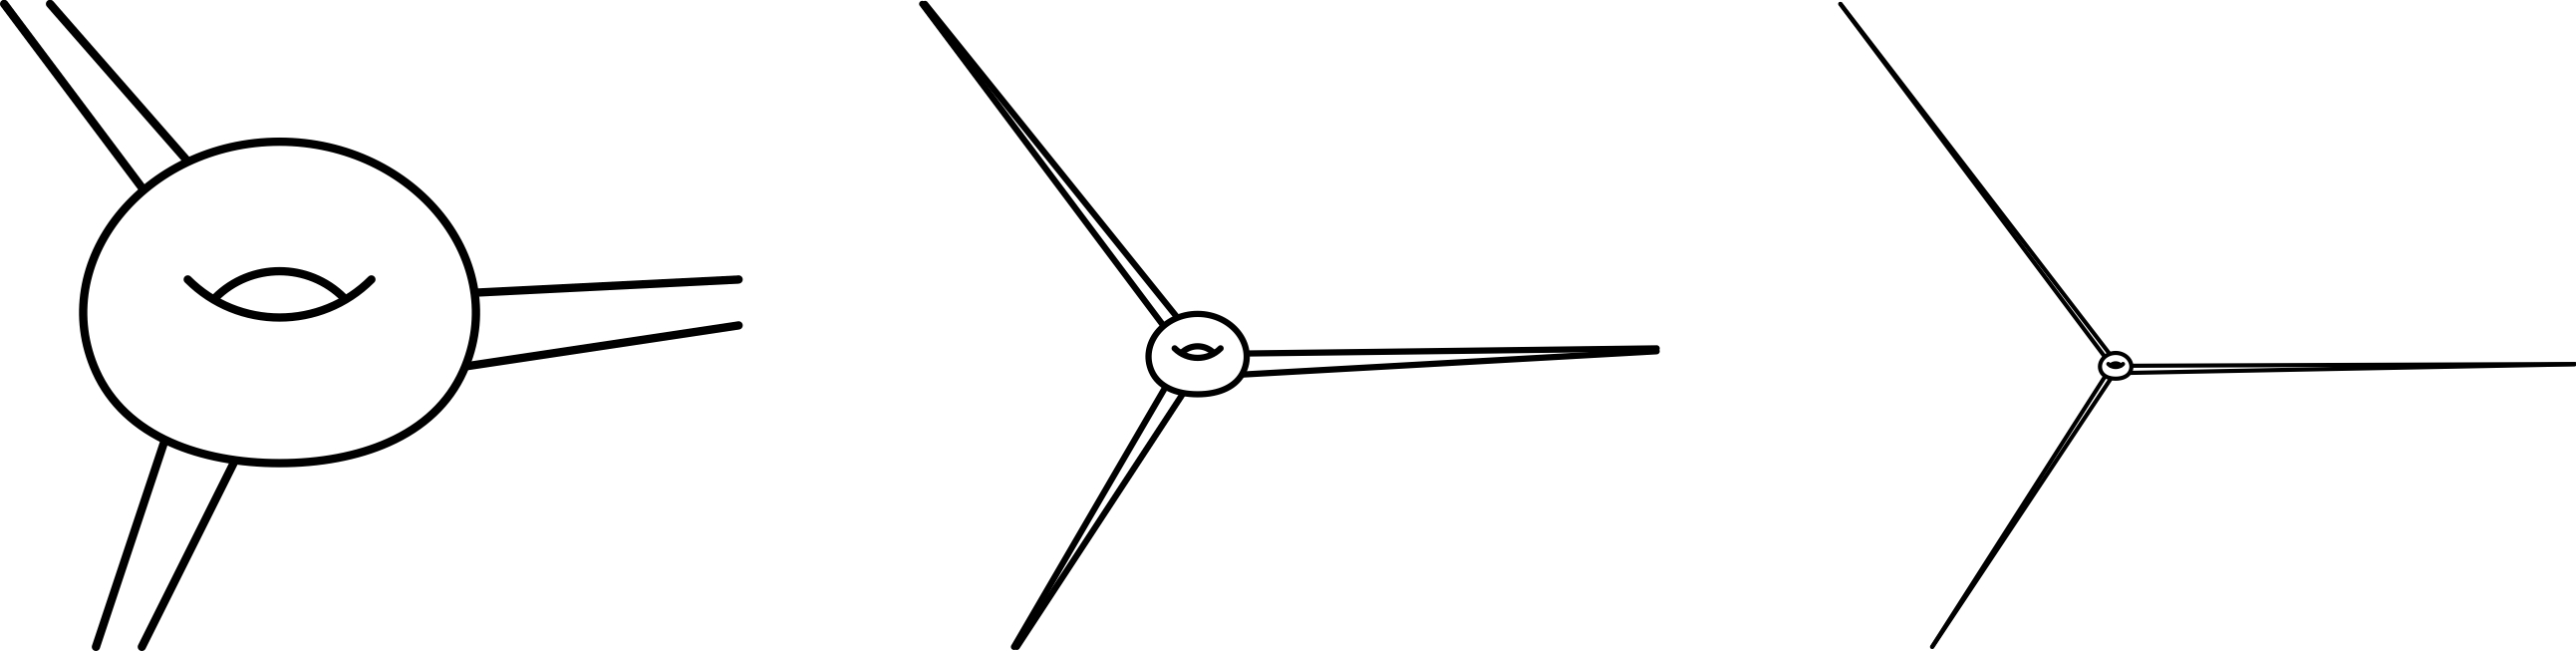
\includegraphics{PDF/shrinkcusps.jpg}}
 \caption{Looking at a manifold with cusps from farther and farther
away.}
 \label{shrinkcusps}
 \end{figure}
%texpreamble
%("  \usepackage{amsmath}
% \usepackage[LY1]{fontenc}
% \usepackage[expert,LY1,mylucidascale]{mylucidabr}
% ");
%defaultpen(  fontcommand("\normalfont") + fontsize(10) ); 
%
%from graph access *;
%unitsize(0.39cm);
%
%currentpen = linewidth(1.25);
%
%void hole(real x, real s) {
%	draw( (x+s,s){SW}..{NW}(x-s, s) );
%	draw( (x+s*0.7,s*0.8){NW}..{SW}(x-s*0.7, s*0.8) );
%	}	
%
%
%void M(real m, real s, real thickness){
%	currentpen = linewidth(thickness);
%	draw( (m-3, 4)..(m,0) ); draw( (m-3+0.5*s^2, 4)..(m+s,0) );
%	draw( (m-2, -3)..(m-s,0) ); draw( (m-2+0.5*s^2, -3)..(m,0) );
%	draw( (m+5, s)..(m,0.75*s) ); draw( (m+5, s - 0.5*s^2)..(m,0.75*s-s) );
%
%	fill( shift(m,0)* (scale(s)*((0,-1){W}..(-2,0)..(0,2.5)..(2,0)..cycle )), white);
%	draw( shift(m,0)* (scale(s)*((0,-1){W}..(-2,0)..(0,2.5)..(2,0)..cycle )));
%	hole(m,s);
%	}
%
%M(0, 1, 1); 
%M(10, 0.25, 0.75);
%M(20, 0.08, 0.5);

\begin{thm}[\csee{LargeScaleRems}] \label{HattoriThm}
 The asymptotic cone of\/ $\Gamma \backslash X$ is a
simplicial complex whose dimension is\/ $\Qrank\Gamma$.
 \end{thm}

\begin{eg} \label{TanConeSL3Z}
 Let $G = \SL(3,\real)$ and $\Gamma = \SL(3,\integer)$. From
\cref{HattoriThm}, we see that the asymptotic cone of
$\Gamma \backslash G/K$ is a $2$-dimensional simplicial complex. In
fact, it turns out to be (isometric to) the sector
 $$ \bigset{ (x,y) \in \real^2 }{ 0 \le y \le \frac{\sqrt{3}}{2} x }
 .$$
 (It is not a coincidence that this sector is a Weyl chamber of
the Lie algebra $\LieSL(3,\real)$.)
 \end{eg}

\begin{rems} \ 
\noprelistbreak
 \begin{enumerate}
 \item If $\Qrank \Gamma = 1$, then the asymptotic cone of
$\Gamma \backslash X$ is a star of finitely many rays emanating from the
origin \fullccf{TanConeEgs}{rank1}. Note that this intersects the unit sphere
in finitely many points.
 \item In general, if $\Qrank \Gamma = k$, then  the unit sphere
contains a certain simplicial complex~$\mathcal{T}_\Gamma$ of dimension
$k - 1$, such that the asymptotic cone of $\Gamma \backslash X$
is the union of all the rays emanating from the origin that pass
through~$\mathcal{T}_\Gamma$.
 \item For $\Gamma = \SL(3,\integer)$, the simplicial
complex~$\mathcal{T}_\Gamma$ is a single edge \ccf{TanConeSL3Z}. In
general, the \term{Tits building}~$\mathcal{T}_G$ is a certain
simplicial complex defined from the parabolic $\rational$-subgroups
of~$G$, and $\mathcal{T}_\Gamma$ can be obtained from~$\mathcal{T}_G$ by
modding out the action of~$\Gamma$.
\item The asymptotic cone is also known as ``\index{tangent cone at infinity|indsee{asymptotic cone}}{tangent cone at infinity}\zz.''
 \end{enumerate}
 \end{rems}

\begin{rem} \label{BScohodim}
Although we will not prove this, the $\rational$-rank is directly reflected in the cohomology of $\Gamma \backslash X$. Namely, let $c$ be the cohomological dimension of $\Gamma \backslash X$. Because 
$\Gamma \backslash X$ is a manifold of dimension $\dim X$, we have 
 $c = \dim X$ if and only if $\Gamma \backslash X$ is compact. So the deficiency $\dim
X - c$ is, in some sense, a measure of how far $\Gamma \backslash X$ is
from being compact. This measure is precisely $\Qrank\Gamma$ (if $X$ has no compact factors).
\end{rem}

%\begin{thm} \label{}
% Assume $X$ has no compact factors. Then the cohomological dimension of
%$\Gamma \backslash X$ is $(\dim X) - \bigl(\Qrank\Gamma \bigr)$.
% \end{thm}


\begin{exercises}

\item \Cref{Qrank0<>cocpct} states that if $\Gamma
\backslash X$ is compact, then $\Qrank \Gamma = 0$.
	\begin{enumerate}
	\item Prove this directly from \fullcref{QrankFlats}{exists}.
	\item Prove this directly from \fullcref{QrankFlats}{BddDist}.
	\end{enumerate}

\end{exercises}




\begin{notes}

Helgason's book \cite{HelgasonBook} has a thorough treatment of
rank and $\real$-rank.

\fullCref{QrankFlats}{BddDist} was proved by B.\,Weiss \cite{Weiss-Qrank}.

\Cref{Qrank0<>cocpct} was proved  for arithmetic lattices by
Borel and Harish-Chandra \cite{BorelHarishChandra} and, independently, by
Mostow and Tamagawa \cite{MostowTamagawa}. For non-arithmetic lattices, this theorem is part of the \emph{definition} of $\rational$-rank.

A more precise version of \cref{HattoriThm} (providing a
description of the geometry of the simplicial complex) was proved by
Hattori \cite{Hattori}. 
Proofs also appear in \cite{JiMacpherson-GeomCpct} and~\cite{Leuzinger-TitsGeom}.

 \Cref{BScohodim} is due to Borel and Serre
\cite{BorelSerre-corners}.

\end{notes}




\begin{references}{9}

\bibitem{BorelHarishChandra}
 A.\,Borel and Harish-Chandra:
 Arithmetic subgroups of algebraic groups,
 \emph{Ann. Math.} (2) 75 (1962) 485--535.
 \MR{0147566},
 \maynewline
 \url{http://dx.doi.org/10.2307/1970210}

\bibitem{BorelSerre-corners}
 A.\,Borel and J.--P.\,Serre:
 Corners and arithmetic groups,
 \emph{Comment. Math. Helvetici} 48 (1973) 436--491.
\MR{0387495},
\maynewline
\url{http://dx.doi.org/10.5169/seals-37166}

\bibitem{Hattori}
 T.\,Hattori:
 Asymptotic geometry of arithmetic quotients of symmetric spaces.
 \emph{Math. Z.} 222 (1996) 247--277. 
 \MR{1429337},
 \maynewline 
 \url{http://eudml.org/doc/174884}
 %\url{http://www.digizeitschriften.de/dms/resolveppn/?PPN=GDZPPN002445301}

\bibitem{HelgasonBook}
 S.\,Helgason:
 \emph{Differential Geometry, Lie Groups, and Symmetric Spaces.}
 Academic Press, New York, 1978.
% (The American Mathematical Society issued a revised edition.) % @@@
\MR{0514561}

\bibitem{JiMacpherson-GeomCpct}
L.\,Ji and R.\,MacPherson:
Geometry of compactifications of locally symmetric spaces,
\emph{Ann. Inst. Fourier (Grenoble)} 52 (2002) 457--559. 
\MR{1906482}, 
\url{http://eudml.org/doc/115986}

\bibitem{Leuzinger-TitsGeom}
E.\,Leuzinger:
Tits geometry, arithmetic groups, and the proof of a conjecture of Siegel,
\emph{J. Lie Theory} 14 (2004) 317--338.
\MR{2066859},
\url{http://www.emis.de/journals/JLT/vol.14_no.2/6.html}

\bibitem{MostowTamagawa}
 G.\,D.\,Mostow and T.\,Tamagawa:
 On the compactness of arithmetically defined homogeneous
spaces,
 \emph{Ann. Math.} 76 (1962) 446--463.
 \MR{0141672},
 \maynewline
 \url{http://dx.doi.org/10.2307/1970368}

%\bibitem{TomanovWeiss}
% G.\,Tomanov and B.\,Weiss:
% Closed orbits for actions of maximal tori on homogeneous
%spaces
% (preprint, 2001).

\bibitem{Weiss-Qrank}
B.\,Weiss:
Divergent trajectories and $\rational$-rank,
\emph{Israel J. Math.} 152 (2006), 221--227.
\MR{2214461},
\maynewline
\url{http://dx.doi.org/10.1007/BF02771984}

 \end{references}
